\documentclass[conference,letterpaper]{IEEEtran}

\ifCLASSINFOpdf
  \usepackage[pdftex]{graphicx}
  \graphicspath{{images/}{figures/}}
  \DeclareGraphicsExtensions{.pdf,.jpeg,.png}
\else
  \usepackage[dvips]{graphicx}
  \graphicspath{{figures/}}
  \DeclareGraphicsExtensions{.eps}
\fi
\newcommand{\subparagraph}{}

\newtheorem{definition}{Definition}
\newtheorem{property}{Property}
\newtheorem{theorem}{Theorem}

\usepackage{amsmath}
\usepackage{color}
\usepackage{xcolor}
\usepackage{colortbl}
\usepackage{listings}
\usepackage{multirow}
\usepackage{mdframed}
\usepackage{url}
\usepackage[subsubsection]{algorithm}
\usepackage{algpseudocode}
\usepackage{lipsum}

\definecolor{LightCyan}{rgb}{0.88,1,1}
\definecolor{BluishGray}{RGB}{226,227,231}
\definecolor{LightGray}{gray}{0.95}
\definecolor{Gray}{gray}{0.85}
\usepackage{amsthm}
%\usepackage{enumitem}
\usepackage[numbers,sort&compress]{natbib}

\theoremstyle{plain}

\theoremstyle{definition}
\newtheorem{defn}{Definition}
\newcommand{\ti}{\textit}
\newcommand{\tb}{\textbf}

\lstset{
language=Ada,                % choose the language of the code
basicstyle=\footnotesize,       % the size of the fonts that are used for the code
%numbers=left,                   % where to put the line-numbers
%numberstyle=\footnotesize,      % the size of the fonts that are used for the line-numbers
%stepnumber=1,                   % the step between two line-numbers. If it is 1 each line will be numbered
%numbersep=5pt,                  % how far the line-numbers are from the code
backgroundcolor=\color{white},  % choose the background color. You must add \usepackage{color}
showspaces=false,               % show spaces adding particular underscores
showstringspaces=false,         % underline spaces within strings
showtabs=false,                 % show tabs within strings adding particular underscores
%frame=single,           % adds a frame around the code
tabsize=2,          % sets default tabsize to 2 spaces
captionpos=b,           % sets the caption-position to bottom
breaklines=true,        % sets automatic line breaking
breakatwhitespace=false,    % sets if automatic breaks should only happen at whitespace
escapeinside={\%*}{*)},          % if you want to add a comment within your code
numbers=right,
numbersep=-10pt,
numberstyle=\tiny,
}

\algrenewcommand{\alglinenumber}[1]{\scriptsize#1:}

\makeatletter
\renewcommand{\ALG@beginalgorithmic}{\scriptsize}
%\renewcommand{\thealgorithm}{\arabic{section}.\arabic{algorithm}}
%\newcommand{\darkalglinenocolor}{%
%   \alglinenumber[1]{\color{black}\footnotesize#1:}}
%%  \setcolor{ALG@color}{\color{black}}}
\makeatother

\begin{document}

\title{Model-driven development and traditional coding - Mind the gap!}

\author{
	\IEEEauthorblockN{Van Cam Pham, Shuai Li, Ansgar Radermacher, Sébastien Gérard, Chokri Mraidha, Rémi Schnekenburger}
	\IEEEauthorblockA{CEA, Address\\
		Email: \{first-name\}.\{last-name\}cea.fr}
}

\maketitle

% TODO This needs to be updated according to the intro!!!

\begin{abstract}
Model-driven engineering (MDE) is a development methodology aiming to increase software productivity and quality by automatically generating code from higher level abstraction models. Although many tools and research prototypes can generate executable code from models such as UML, generated code could be manually modified by programmers. After code modifications, round-trip engineering (RTRIP) supported by many tools is needed to make the model and code consistent but most of the tools are only applicable to static diagrams such as classes. In this paper, we address the RTRIP of UML State Machine diagrams and code. We propose a RTRIP approach consisting of a forward process, which generates code, and a backward process, which updates the original state machine from the modified generated code. From the proposed approach, we implemented a prototype and conducted several experiments on different aspects of the round-trip engineering to verify the proposed approach.
\end{abstract}


%\begin{IEEEkeywords}
%Key words
%\end{IEEEkeywords}

%\thispagestyle{plain}
%\pagestyle{plain}

%Some terms to find, define, and keep coherent:
%- Developer
%- The developer who uses models is called... (e.g. software architect modeler? doesn't mean anything)
%- The developer who uses code is called... (e.g. programmer)
%- Our method is for... called... (e.g. method for model code synchronization, method for architect/programmer collaboration, etc...)
%- Model is...
%- Code is...
%- Gap or difference ?
%- Background or practice or habits or profiles ? Maybe keep profile and choose one of the other?


\section{Introduction}
\label{sec:introduction}
Model-driven engineering (MDE) is a development methodology aiming to increase software productivity and quality by allowing different stakeholders to contribute to the system description \cite{Mussbacher2014}. MDE considers models as first-class artifacts and generates code from higher abstraction level models. Although many tools and research prototypes can generate executable code from models such as UML \cite{Specification2007}, generated code could be manually modified by programmers, e.g. skeleton code generated from UML class diagrams. Models and the generated code are therefore out of synchronization. Round-trip engineering is proposed to keep the artifacts synchronized.

Round-trip engineering \cite{Aßmann200333} (RTRIP) supports synchronizing different software artifacts, model and code in this case, and thus enabling actors (software architect and programmers) to freely move between different representations \cite{Sendall}. Tools such as for instance Enterprise Architect \cite{sparxsystems_enterprise_2014}, Visual Paradigm \cite{visual}, AndroMDA \cite{_andromda_} provide RTRIP but most of them are only applicable for system structure models such as class diagrams. The RTRIP of behavior diagrams is simply not supported by these tools since (1) RTRIP is a challenge even for structural code and there is a (2) the gap between behavior models and low level code. There are no obvious bijective mappings from behavioral models and code. Furthermore, user modifications made to the generated code are not trivial to control and reflect to the model.

This study addresses the RTRIP of UML State Machine (SM) and object-oriented programming languages such as C++ and JAVA. SM is widely used in practice for modeling the behavior of complex systems, notably reactive, real-time embedded systems. There are several approaches to generating source code from state machines or state charts such as nested switch/if statements \cite{Booch1998}, state-event-table \cite{Douglass1999, Duby2001} approach and state pattern \cite{Allegrini2002,Shalyto2006,Douglass1999}. Unfortunately, the generated code from these approaches is very difficult for programmers to maintain without an appropriate supporting tool. RTRIP is impossible in these approaches even with very small changes such as changing transition targets or actions made to code. The reason behind this impossibility is that, in mainstream programming languages such as C++, JAVA, there are not equivalents between SM and source code statements.

Synchronization of SM and code allows stakeholders to better collaborate in reactive software system development. In this paper, we propose an approach to supporting this synchronization. The approach consists of a forward and a backward process. The forward process taking as input a SM executes two transformations. The first is UML to UML by utilizing several transformation patterns such as the double-dispatch approach presented in \cite{spinke_object-oriented_2013} and the second is a generation of code from the transformed UML. During the transformations, traceability information is stored. In the backward direction, a verification is executed by code pattern detection to verify the static semantic correctness of the code before the backward process taking as input the modified generated code, the UML classes, the original SM and mapping information together merges changes from code to the SM. From the proposed approach, we implemented a prototype supporting RTRIP of SM and C++ code, and conducted several experiments on different aspects of the RTRIP to verify the proposed approach. Our implementation is the first tool supporting RTRIP of SM and code. 
%The prototype also improves the collaboration between MDE developers and traditional programmers in developing reactive complex embedded systems.

To sum up, our contribution is as followings:
\begin{itemize}
  \item An approach to round-tripping UML SMs and object-oriented code.
  \item A first tooling prototype supporting RTRIP of UML SMs and C++ code.
  \item An automatic evaluation of RTRIP correctness of the proposed approach with the prototype including 300 random generated SM models containing 80 states, more than 230 transitions, more than 250 actions and around 180 events for each.
  \item A complexity analysis of the approach and performance evaluation.
  \item A comparison and collaboration of two software development practices including working at the model level and at the code level.
  \item A lightweight evaluation of the semantic conformance of the runtime execution of generated code.
\end{itemize}

The remaining of this paper is organized as follows: Section \ref{sec:related_works} shows related work. Our proposed approach is detailed in Section \ref{sec:approach}. The implementation of the prototype is described in Section \ref{sec:implementation}. Section \ref{sec:experiments} reports our results of experimenting with the implementation and our approach. The conclusion and future work are presented in Section \ref{sec:conclusion}.


\section{Related Work}
\label{sec:related_works}
Two main topics directly related to our study are identified. One is the implementation techniques and code generation for UML SMs and the other one is RTRIP.
\subsection{Implementation and code generation for UML SMs}
Main approaches including switch/if, state table and state pattern are investigated.

Switch/if is the most intuitive technique implementing a "flat" state machine. Two types of switch/if are supported. The first one uses a scalar variable representing the current active state \cite{Booch1998}. A method for each event processes the variable as a discriminator in switch/if statement. The second one uses doubly nested switch/if and has two variables to represent the current active state and the event to be processed \cite{Douglass1999}. The latter are used as the discriminators of an outer switch statement to select between states and an inner one/if statement to decide how the event should be processed. The behavior code of the two types is put in one file or class. This practice makes code cumbersome, complex, difficult to read and less explicit when the number of states grows or the state machine is hierarchical. Furthermore, the first approach lets the code scatter in different places. Therefore, maintaining or modifying such code of complex systems is very difficult.

In \cite{Douglass1999, Duby2001} the authors also propose a double dimensional state table in which one dimension represents states and the other one all possible events. Each cell of the table is associated with a function pointer meaning that the state associated with a dimension index of the cell is triggered by the event associated with the other dimension. This technique is efficient for flat and simple state machines. As the switch/if technique, this approach gets cumbersome and non-trivial to maintain since states and events represented by indexes of the table are not explicit. Furthermore, this approach requires every transition must be triggered by at least an event. This is obviously only applied to a very small sub-set of UML state machines.  
  
State pattern \cite{Allegrini2002,Shalyto2006,Douglass1999} is an object-oriented way to implement state machines. Each state is represented as a class and each event as a method. The event processing is executed by a delegation from the state machine context class to sub-states. Separation of states in classes makes the code more readable and maintainable. Unfortunately, this technique only supports flat state machines. The authors in \cite{niaz_mapping_2004} extends this to overcome its limitations. However, the maintenance of the code generated or implemented by this approach is not trivial since it requires a lot of code to write and many small changes in different places. This is critically impractical when dealing with large state machines. Furthermore, similar to the state table, this approach also poses the requirement of having at least one event for transition.

Double-dispatch pattern is proposed in \cite{spinke_object-oriented_2013} as a new technique to implement state machines. States and events are represented as classes. Our generation approach relies on this approach. The latter provides some 1-1 mappings from state machines to object-oriented code and the implementation technique is not dependent on a specific programming language. However, the approach does not deal with triggerless transitions and different event types supported by UML such as \ti{CallEvent}, \ti{TimeEvent} and \ti{SignalEvent}. Furthermore, the proposed approach is not a code generation approach but manual implementation.

Readers of this paper are recommended referring to c\cite{Domnguez2012} for a systematic survey on different approaches generating code from state machine/state charts.

\subsection{Round-trip engineering}
RTRIP of UML models and object-oriented code are supported in many tools including research prototypes and commercial such as Enterprise Architect \cite{sparxsystems_enterprise_2014}, Visual Paradigm \cite{visual}, AndroMDA \cite{_andromda_}. Although these tools work well with UML class diagrams and code, behavioral diagrams are not well supported.  

Fujaba \cite{KNNZ99_2_ag} offers a round-trip engineering environment. An interesting part of Fujaba is that it abstracts from Java source code to UML class diagrams and a so-called story-diagrams. Java code can also be generated from these diagrams. RTRIP of these diagrams and code works but limited to the naming conventions and implementation concepts of Fujaba which are not UML-compliant. 

The authors in \cite{angyal_synchronizing_2008} propose a syntactic synchronization technique for domain-specific modeling languages (DSML) and code. The approach uses an Abstract Syntax Tree (AST) metal-model to model source. Changes in code detected by using an algorithm proposed  in \cite{Chawathe:1996:CDH:235968.233366} to compare the AST instance of the current code with the last synchronized one are merged to the instance of DSML. However, an AST is very low level and it is not clear to have mappings from DSML instances to AST instances. Furthermore, although there is an example for illustrating the technique, a systematic evaluation of the approach is not presented to show its scalability.

%Round-trip engineering of Activity diagram and code is proposed in [13]. The approach uses intermediate models to reduce the abstraction gap between diagrams and code. However, the activity diagram contains plenty of low level information such as variable declarations. Furthermore, no semantic analysis is supported.


\section{Actors and use-cases}
\label{sec:use-case}

In this section we define the actors who will use our method to collaborate.
Then we present the use-cases of a generic development environment used by
the actors. The use-cases are the functionalities that the development environment
must have for model-code synchronization.

\subsection{Actors}

In this paper we propose a method for collaboration between model-driven developers
and code-driven developers, who are thus the actors who will use the proposed method.
Before defining these actors, let us first define the concept of development artifact and reference artifact.

% TODO find standard definition
\begin{definition}[Development artifact]
A development resource is a resource that contains enough information
for the implementation of the system.
\end{definition}

For example a system can be entirely implemented as code.
The code project is then a development artifact.
A model may also be a development artifact.
It is then not only documentation of specification.
For example a model can be used for implementation either by compiling
it directly \cite{asma}, or by generating code from the model, and compiling the code without
the need to modify it.

% TODO find standard definition
\begin{definition}[Reference artifact]
A reference artifact is one which may be modified manually.
All other artifacts are produced from the reference artifact
through some process, and only through the process. Manual modification
of artifacts other than the reference artifact is forbidden.
\end{definition}

The actors who will use our method are called 
model-driven developer and code-driven developers.
Both are developers which is defined as follows:

\begin{definition}[Developer \cite{developer_def_ref}]
TODO: find a definition in standard docu
\end{definition}

The main difference between a model-driven developer and a code-driven developer
is what they consider as the reference artifact.

% TODO find standard definition
\begin{definition}[Model-driven developer]
A model-driven developer is a developer for whom the model is the reference artifact
during development.
\end{definition}

Otherwise said, for the model-driven developer only the model should be modified manually. The
code must always be produced from the model through some process that guarantees that the
code is conform to the model. Note that in the case of an object-oriented model, not only
is the architecture of the project stored in the model, but also the implementation of
methods.

% TODO find standard definition
\begin{definition}[Code-driven developer]
A model-driven developer is a developer for whom the code is the reference artifact
during development.
\end{definition}

\subsection{Use-cases}

In this section we propose a development environment with
use-cases that make it possible for the actors to develop
the system with their development preferences.
Figure \ref{fig:use-case} shows a UML use-case diagram of the development environment
and their associations to the actors. (UML notations are used.)

% TODO: bold text in figure
\begin{figure}
\centering
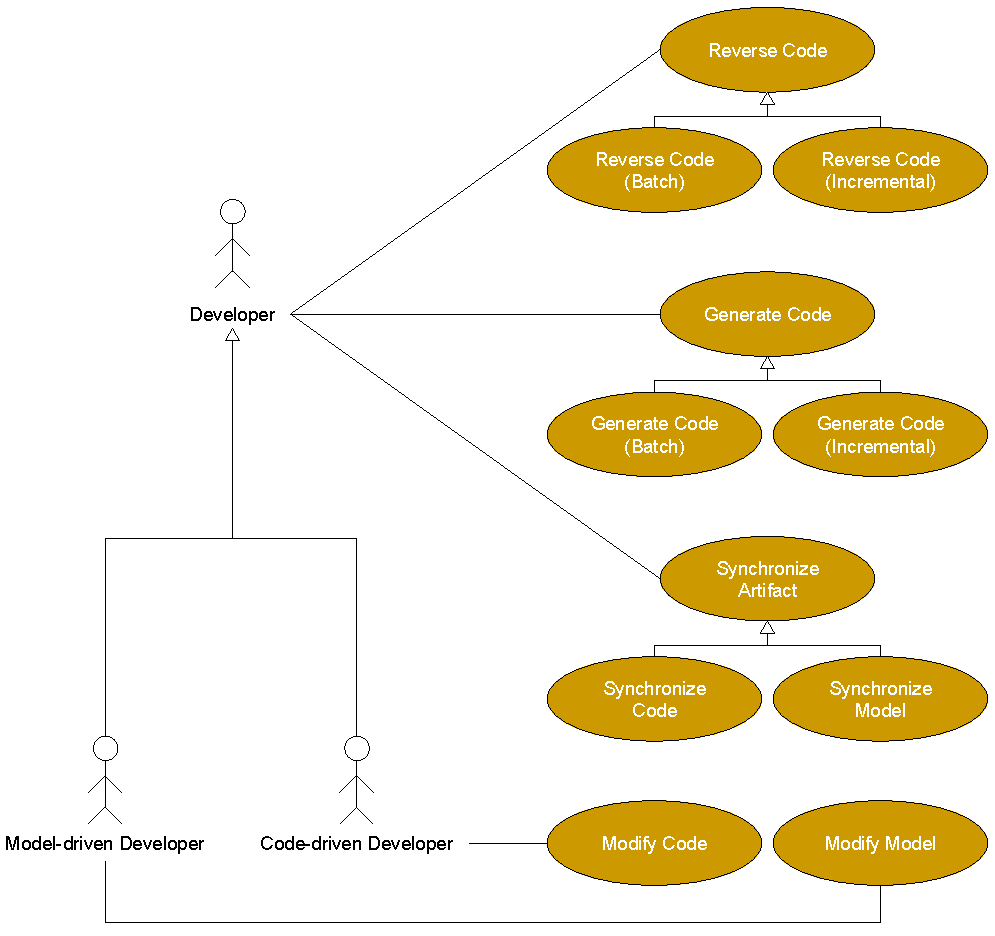
\includegraphics[width=\columnwidth]{figures/use-case}
\caption{Use-case Diagram} 
\label{fig:use-case}
\end{figure}

There are some use-cases for manual modification of artifacts. The \textbf{Modify Artifact} use-case
means the development environment must have some tool to let the developer manually modify an artifact.
The \textbf{Modify Model} and \textbf{Modify Code} use-cases are specializations of the \textbf{Modify Artifact}
use-case where model and code are respectively the artifact in question.

There are also some use-case for the synchronization of artifacts. The \textbf{Synchronize Artifact} use-case
is the synchronization of two artifacts by updating each artifact to reflect changes made to the other artifact,
and by reconciling conflicts between the artifacts. The \textbf{Synchronize Model} and \textbf{Synchronize Code}
use-cases are specializations where model and code are respectively the artifact in question.

Finally there are some use-cases for producing one artifact from the other and vice versa.
The \textbf{Generate Code} use-case is the production of code in a programming language from a model in a modeling language.
This use-case is related to forward engineering \cite{forward_engineering_ref} which is the production
of implementation from specification.
% Do we need this definition of forward engineering? Isn't it more confusion actually since we 'implementation' and 'specification' keywords.
The developer can either use \textbf{Generation Code (Batch)} or \textbf{Generate Code (Incremental)}. Batch
code generation produces new code from the model. If any code existed before, it is overwritten entirely with
the new code. Incremental code generation is [Official definition here].

The \textbf{Reverse Code} use-case is the production of model in a modeling language from code in a programming language.
This use-case is related to \cite{reverse_engineering_ref} which is the production of specification from implementation.
% Do we need this definition of reverse engineering? Same reasons as above.
The developer can either use \textbf{Reverse Code (Batch)} or \textbf{Reverse Code (Incremental)}.
Like their counter-part in the code generation use-cases, the difference between batch and
incremental reverse is the how the produced artifact is updated or overwritten.

\section{Processes to synchronize model and code}
\label{sec:processes}

%Model-driven engineering has been established as a potential approach to gain software quality and productivity \cite{Mussbacher2014}. 
This section shows our use cases and scenarios in the collaboration of model-driven developers and traditional developers. The scenario 1 and 2 show how simple forward and reverse engineering combined to a create a RTE supported by most round-trip engineering tools such as 

\subsection{Scenario 1: modifications only made to code}
\label{scenario1}

The scenario 1 occurs when a group of people consisting of software architects, model-driven developers and traditional developers (programmers) have a need to create a software based on a legacy system or some legacy code that programmers are working with and want to directly contribute to the system description in order to gain quality. In the first step, it is of course not easy to communicate the stakeholders in the group. To have better understanding of the legacy system, a traditional reverse engineering is enough. 

In Fig. \ref{fig:scenario1}, the step (1) is to reverse the legacy code of the legacy system to a model. This scenario has a possible variant in case of not having an existing legacy system and the model is created from scratch. Based on the diagrams rendered the step (1), the stakeholders can discuss the system overall and ask programmers what to do in the legacy code. Nevertheless, this traditional development method does not profit the advantages of Model-driven engineering that allows to generate code and provides better organization. Therefore, we have a step (2) to modifying or re-factoring the created model to have a better architecture of the system and generating code from the model. The programmers then work with this generated code rather than the legacy code in the step (3). The architects and model-driven developers then reverse engineer the evolved code back to the model by an overwriting and analyze the system by using the new model in the step (4). The steps (2) and (4) are supported by many research prototypes and commercial tools \cite{UModel, visual, Rhapsody, Magicdraw, EA} but the model created in the step (4) is usually a surprise to architects since its diagrams are rendered differently from the original model. To handle this problem, it is necessary to preserve diagrams' properties of the original model by an incremental reverse engineering in the step (4) which is limitedly supported by most of the tools. 

\begin{figure}
\centering
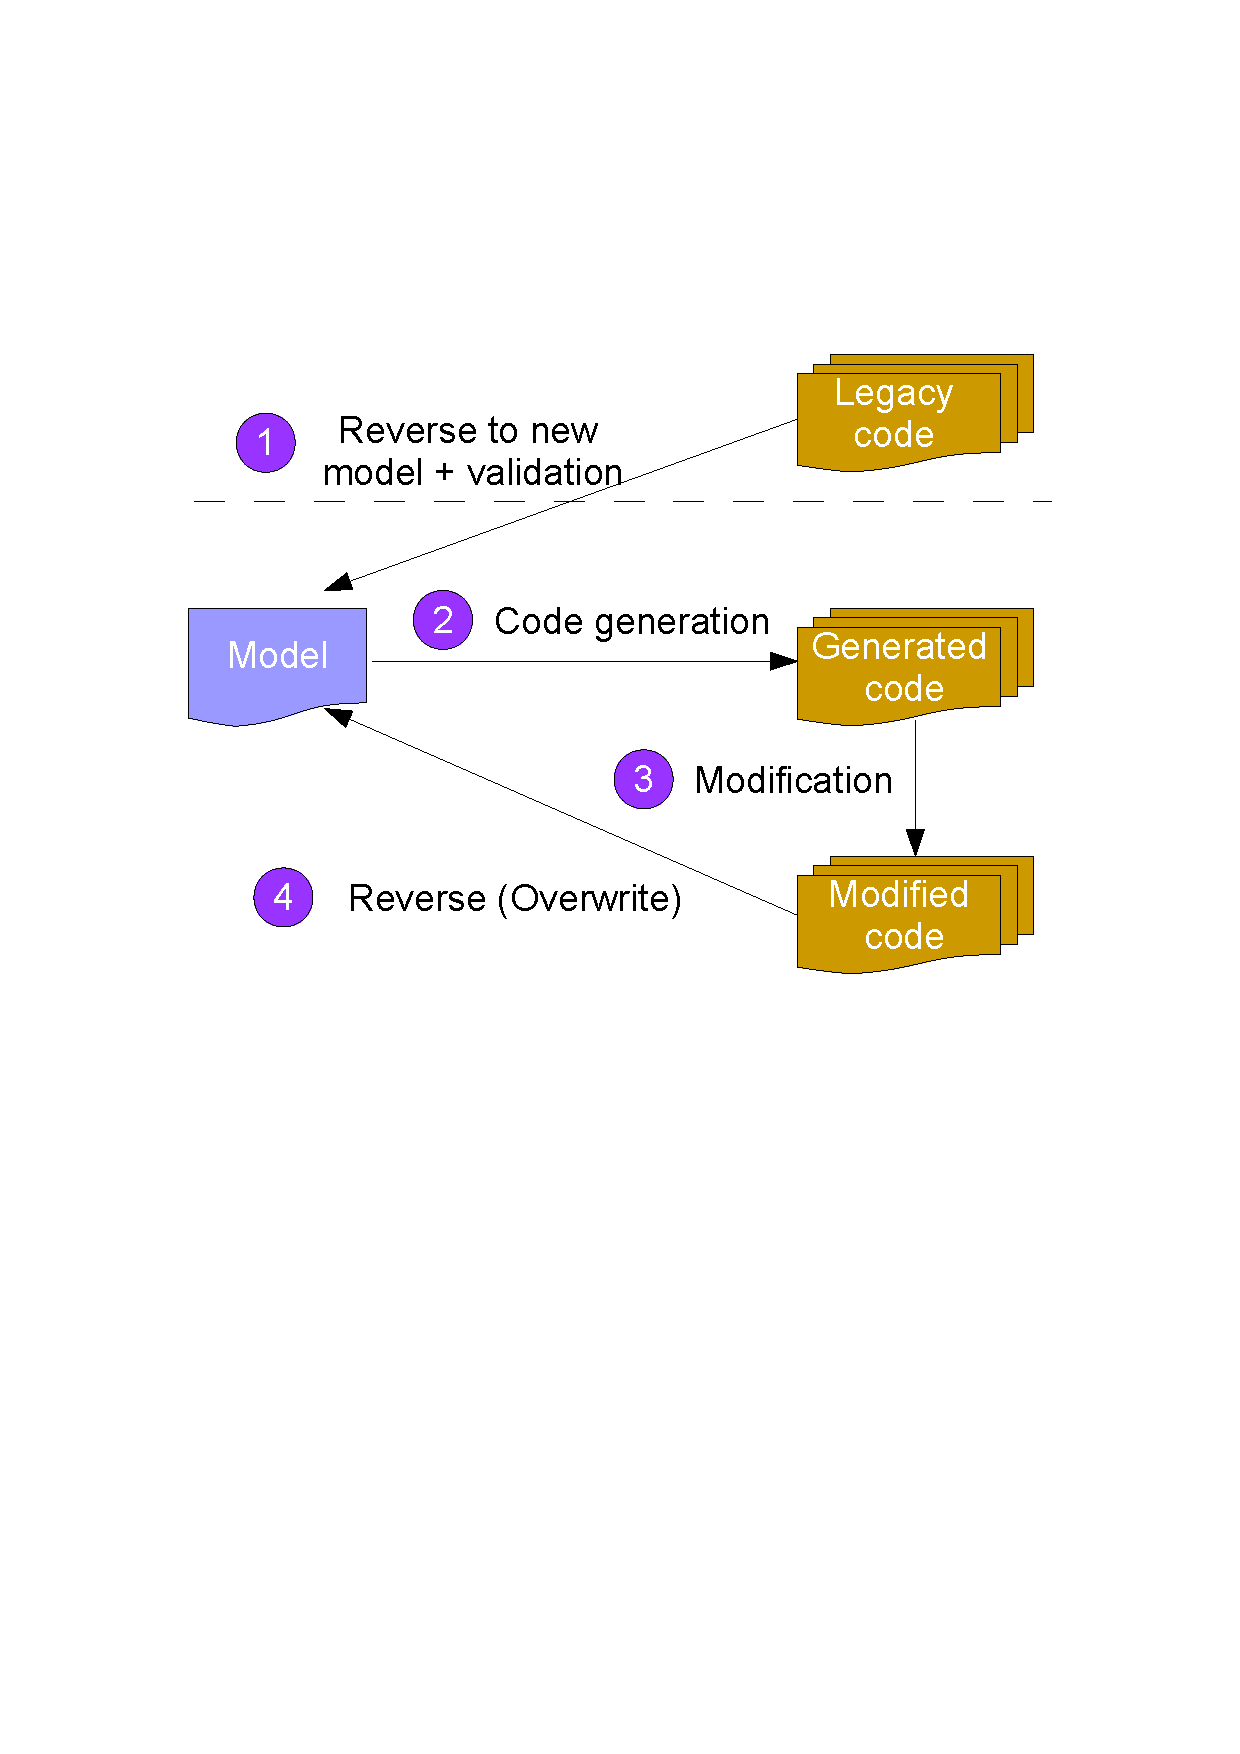
\includegraphics[height = 0.20\textheight, trim = 90 370 60 170, clip]{figures/scenario1}
\caption{\label{fig:scenario1}Round-trip engineering in case only code is modified} 
\end{figure}

\subsection{Scenario 2: modifications only made to model}
\label{scenario2}
The scenario 2 is similar to the scenario 1 in the first two steps (see Fig. \ref{fig:scenario2}. The difference is that instead of changing the generated code, MDE developers make modifications on the model. This scenario is close to re-engineering \cite{Chikofsky1990} of a software system by using MDE paradigm. In order to make the modified model and code consistent again, a code generation is needed in the step (4). The batch generation is supported by many tools as mentioned in the sub-section \ref{scenario1}, incremental code generation is still missing in these tools.  

\begin{figure}
\centering
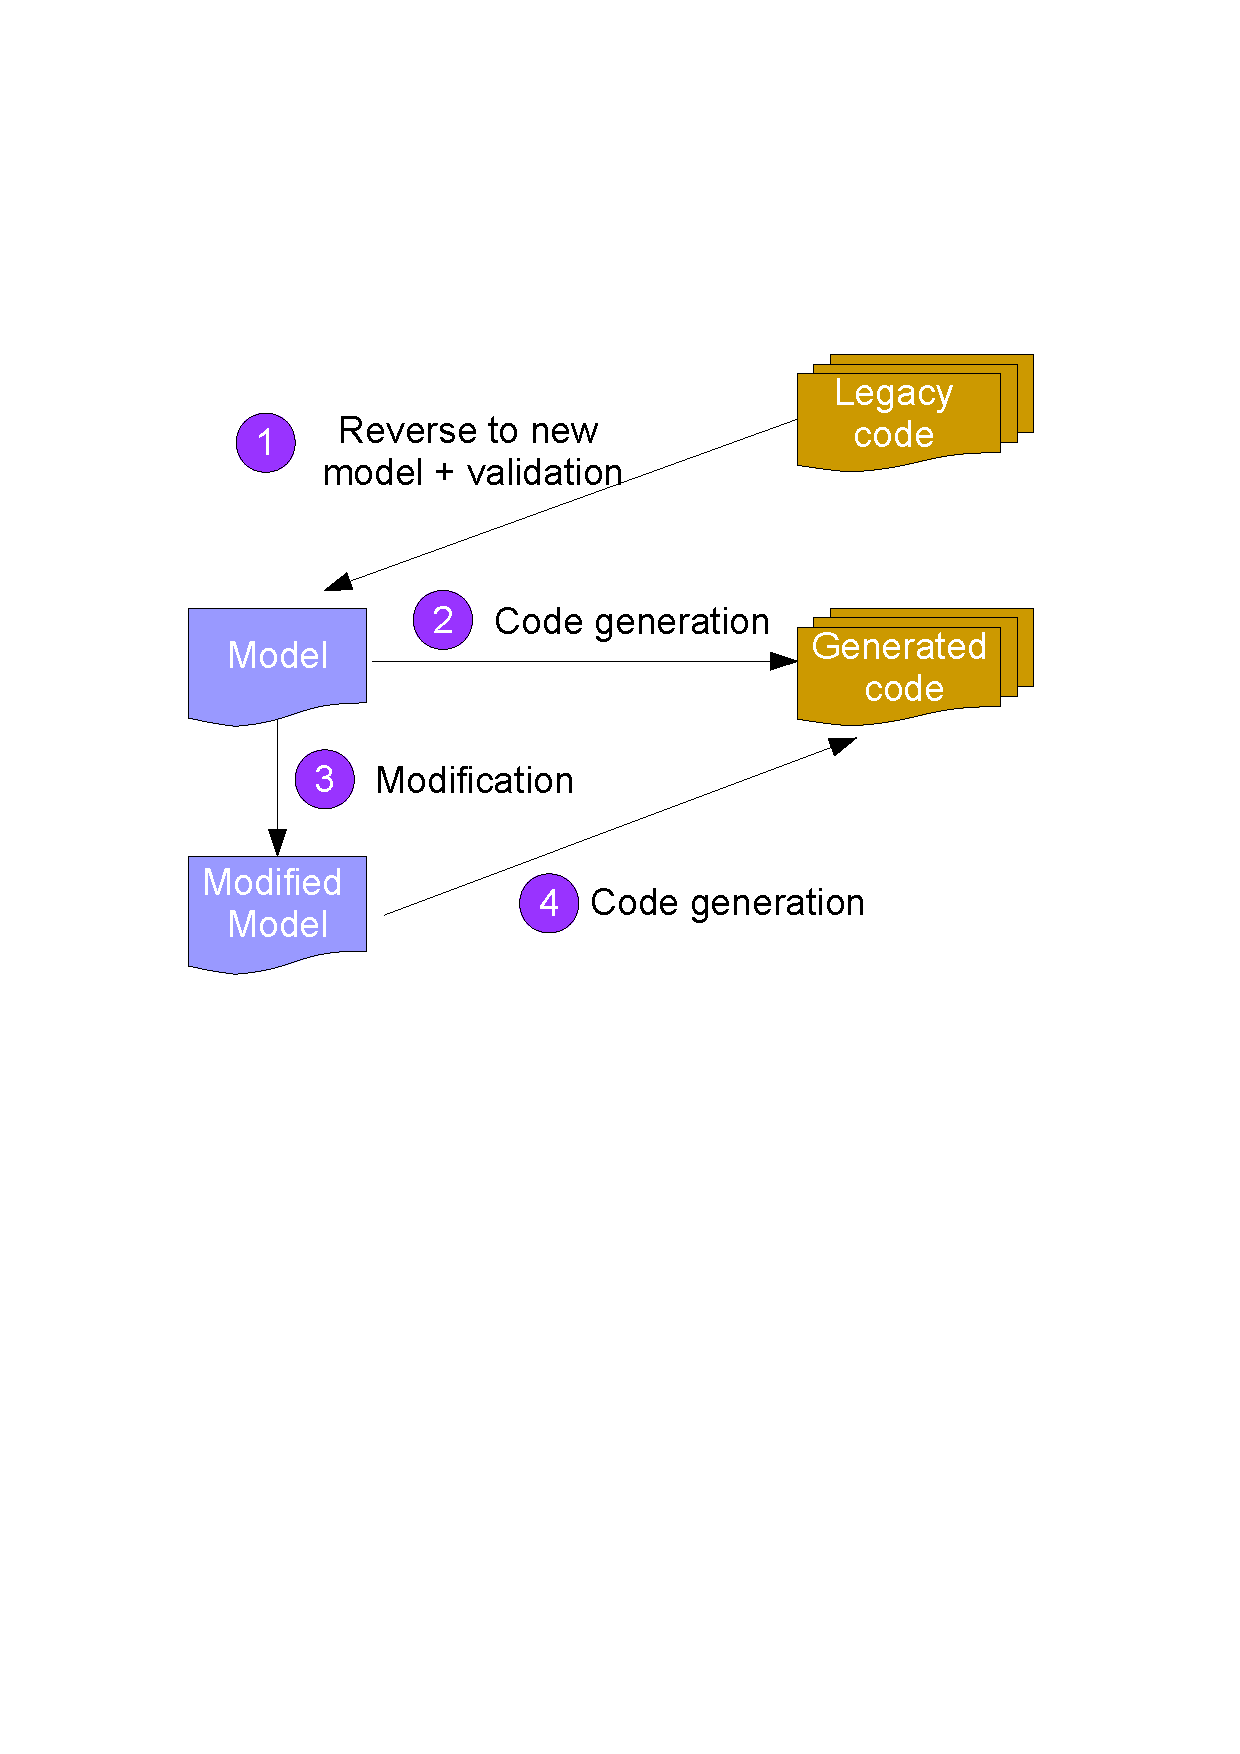
\includegraphics[height = 0.20\textheight, trim = 90 370 60 170, clip]{figures/scenario2}
\caption{\label{fig:scenario2}Round-trip engineering in case only model is modified} 
\end{figure}


\subsection{Scenario 3: concurrent modifications}
\label{scenario3}
The beauty of MDE is that it allows not only programmers but all different stakeholders concurrently contribute to the system description that is in turn translated to code. This ability gains software quality and productivity. This is where the scenario 3 stems from. Let's imagine that after creating software model by reverse engineering in the step (1) in Fig. \ref{fig:scenario3}, software architects may change the system architecture by re-factoring and in the meantime, traditional programmers might delete or add more methods/attributes or simple change methods' behavior. The modified model and code are then out of synchronization. The gap between the model and code makes the two profiles inconsistent: one artifact is non-sense to the other. This inconsistency in turn reduces the software quality. Therefore, a real synchronization is needed in the step (4). 

\begin{figure}
\centering
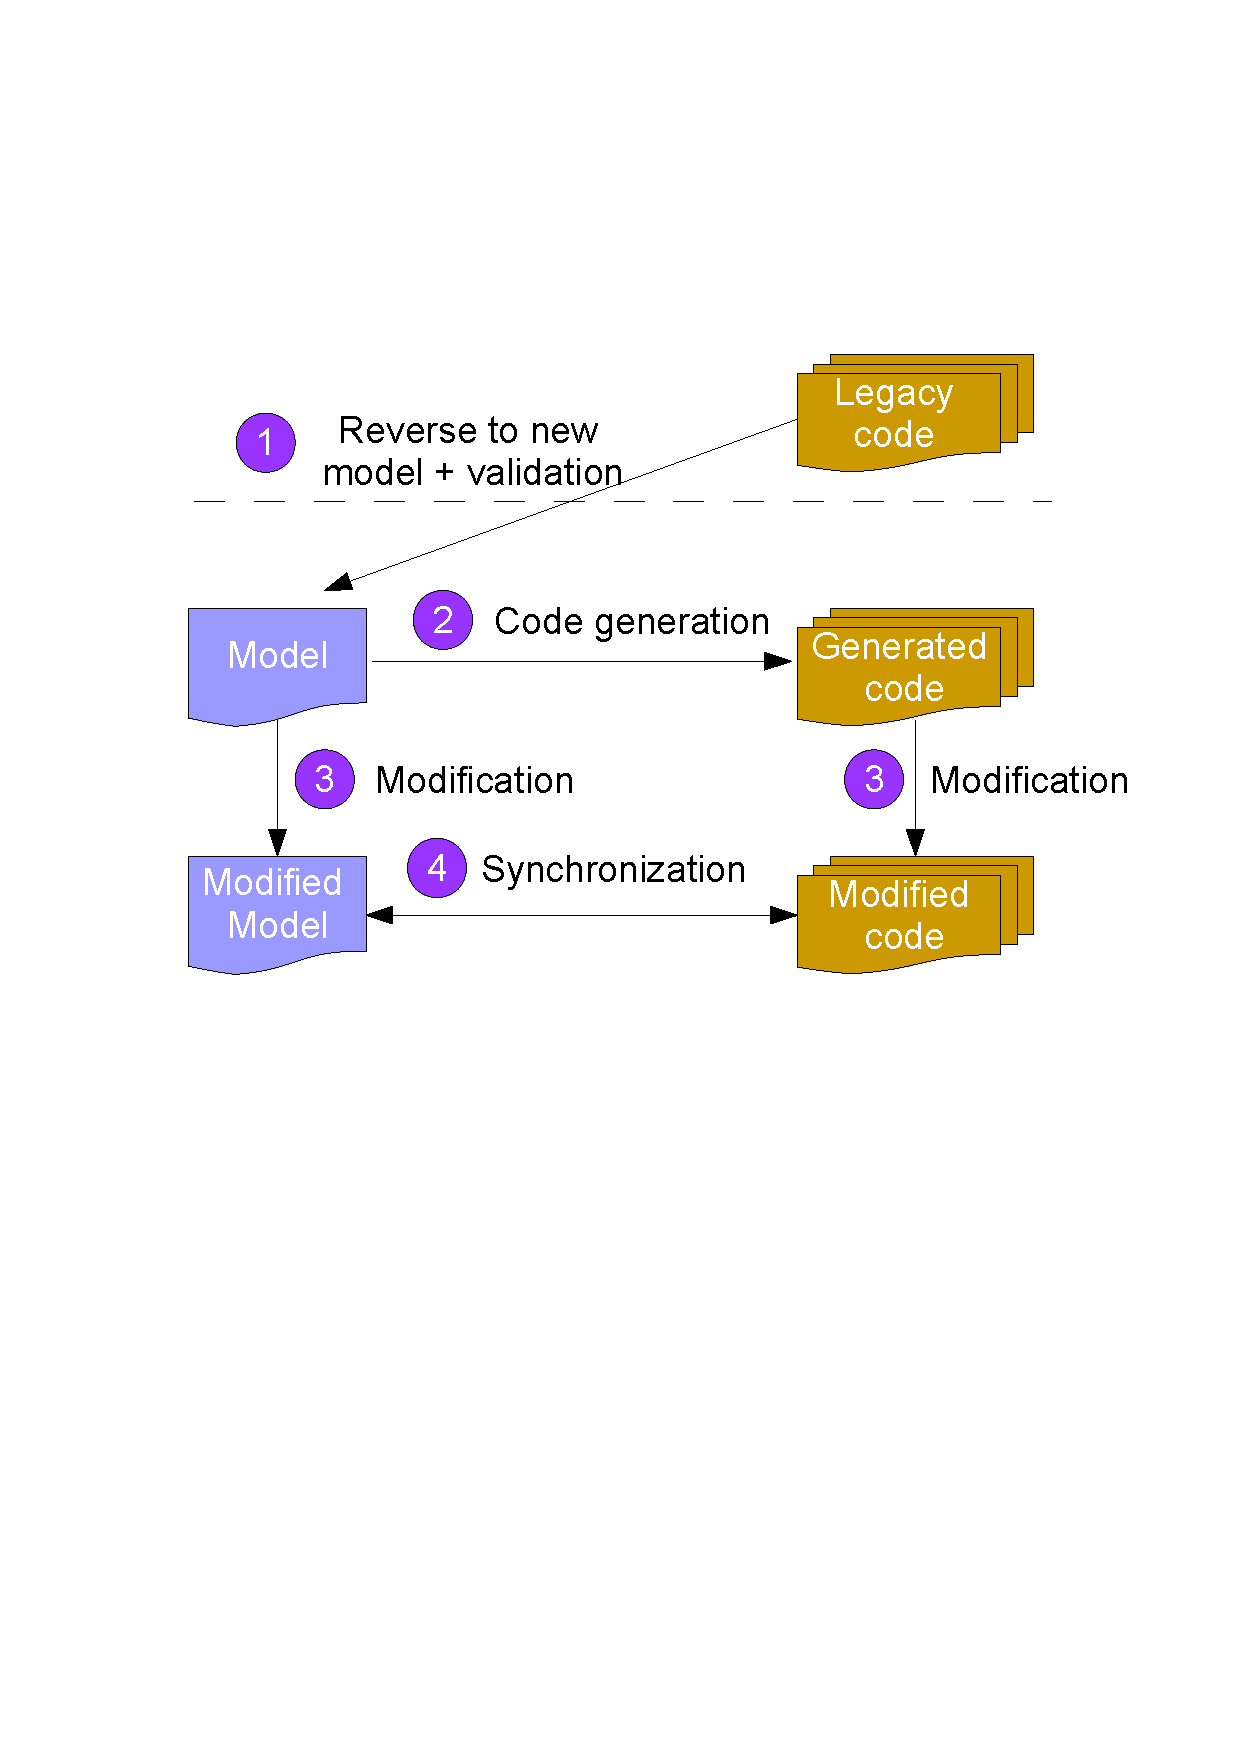
\includegraphics[height = 0.20\textheight, trim = 90 370 60 170, clip]{figures/scenario3}
\caption{\label{fig:scenario3}Model and code are concurrently modified} 
\end{figure}
\section{implementation}
\label{sec:implementation}
The proposed approach is implemented in a prototype existing as an extension of the Papyrus modeler [4]. Each state machine is created by using a state machine diagram and contained in a component. Low-level processing of state machine actions is directly embedded by a block of code written specific programming languages such as C++/JAVA in the state machine. C++ code is generated by the prototype but other object-oriented languages are easily generated. The code generation consists of transforming the state machine to UML classes and eventually to code by a code generator following the proposed approach. In the reverse direction, code pattern detection is implemented as described in the previous section to verify state machine semantics in code. If the generated code is modified, two options are supported by the prototype interface to make the state machine and code consistent again. One is to create a new state machine from the modified code in the same Eclipse project and the other one is to update the original state machine by providing as input the intermediate model and the state machine in a dialog.
\section{Experiments}
\label{sec:experiments}
In order to evaluate the proposed approach and the prototype, we answer two questions related to two laws of RTE \cite{foster_combinators_2007}. 

\tb{RQ1}: A state machine \ti{sm} is used for generating code. The generated code is reversed by the backward transformation to produce another state machine \ti{sm'}. Are \ti{sm} and \ti{sm'} the same? In other words: whether the code generated from UML state machines model can be used for reconstructing the original model.

\tb{RQ2}: A state machine sm is used for generating code. The generated code is modified by adding/deleting/modifying elements such as states, transitions, or events. The modified code is then reversed by merging changes to sm. Are modifications in the modified code propagated to sm?

This section reports our experiments targeting to the two questions. Two types of experiments are conducted. For each type, the number of elements in models are taken into account by a JAVA program. Figure \ref{fig:strategy1} and Figure \ref{fig:strategy2} show the evaluation methodologies to answer \tb{RQ1} and \tb{RQ1}, respectively. Additionally, the time complexity and performance analysis of our approach is also presented. Results of a lightweight experiment on the semantic conformance of runtime execution of the generated code are also shown afterward.

\begin{figure}
\centering
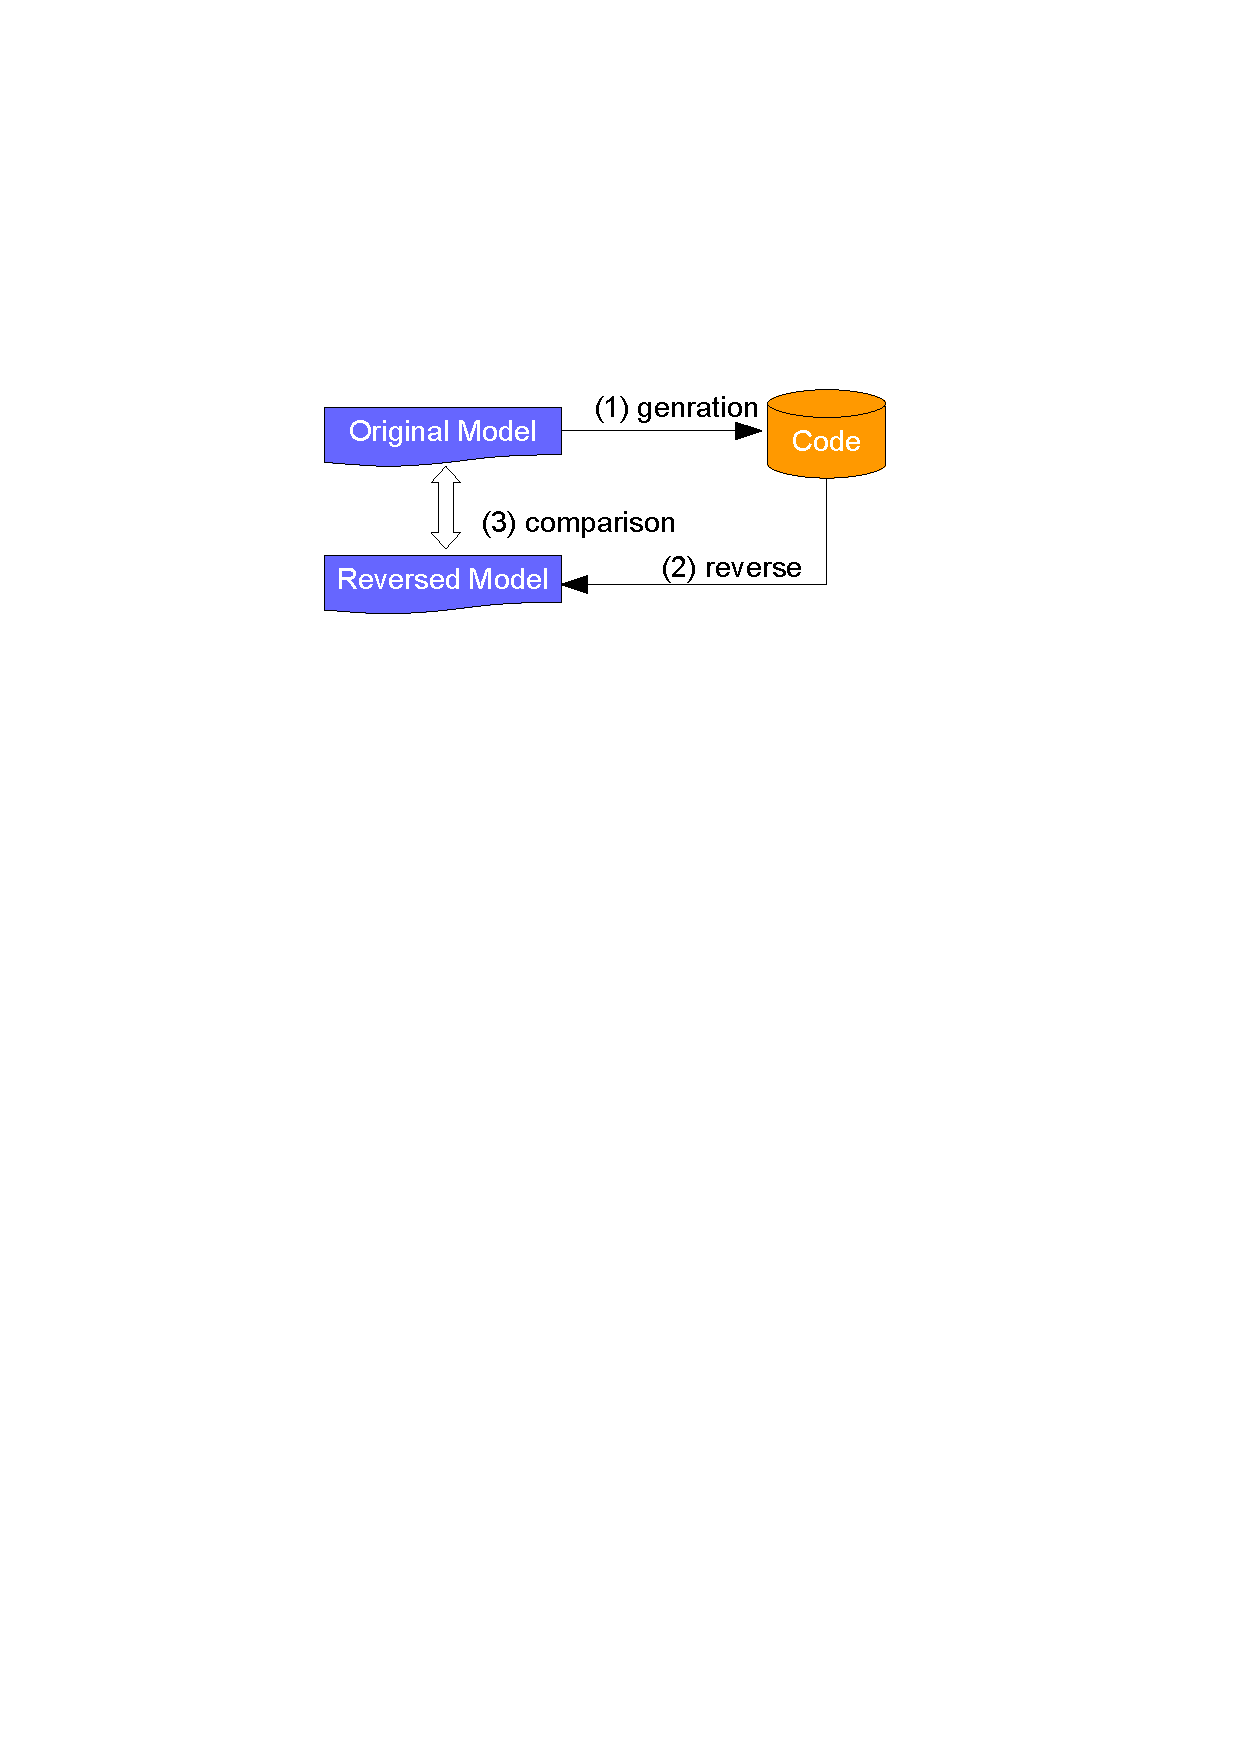
\includegraphics[clip, trim=5.5cm 19cm 5.5cm 6cm, width=0.3\textwidth]{figures/strategy1}
\caption{Evaluation methodology to answer RQ1} 
\label{fig:strategy1}
\end{figure}

\begin{figure}
\centering
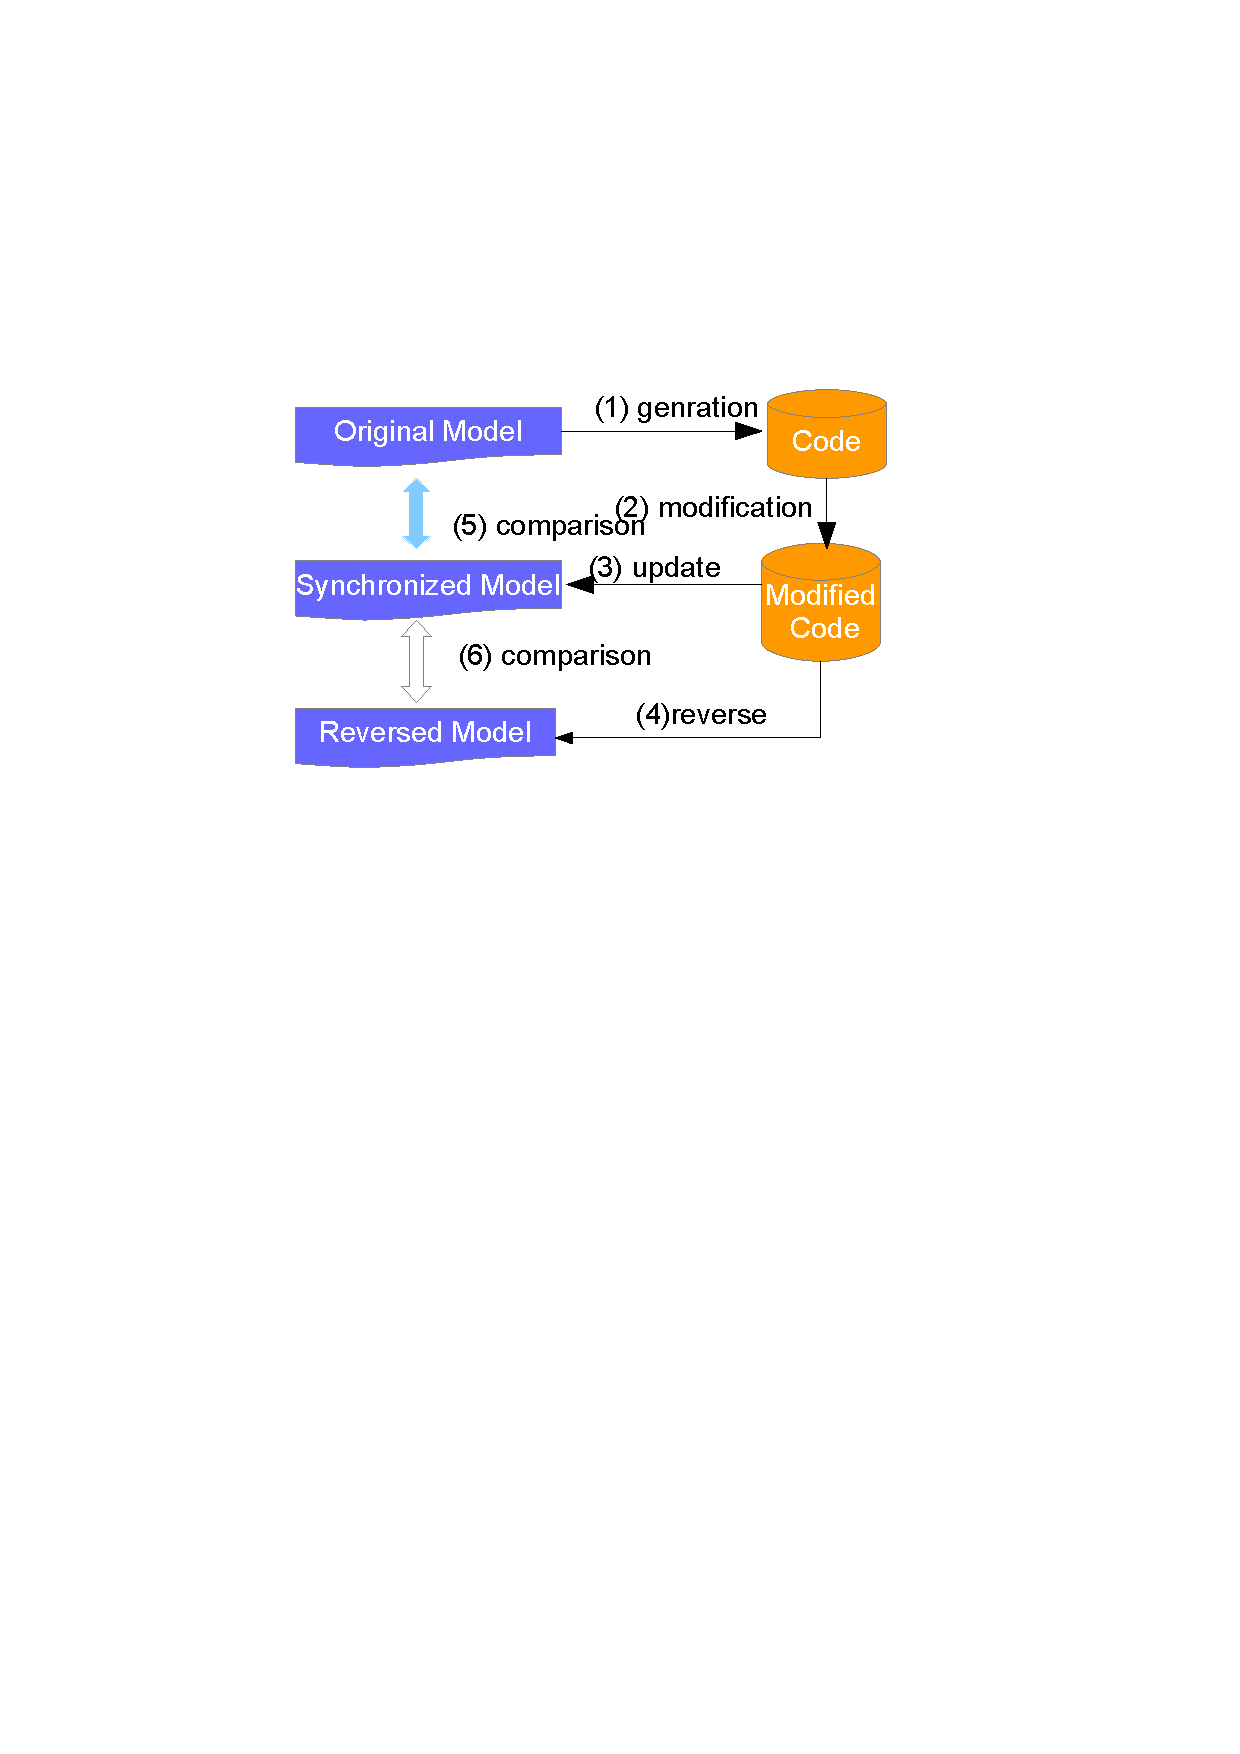
\includegraphics[clip, trim=4.5cm 16.5cm 5.5cm 6.5cm, width=0.3\textwidth]{figures/strategy2}
\caption{Evaluation methodology to answer RQ2} 
\label{fig:strategy2}
\end{figure}

Furthermore, in software development projects, some traditional programmers might want to practice with code in a traditional way and some MDE developers may prefer working with models. Therefore, it is necessary to compare the development/maintenance cost between the two practices by comparing the number of steps needed to do the same action. 


\subsection{Reversing generated code}
This experiment is targeting \tb{RQ1}. 300 hierarchical state machines are randomly automatically generated. Each of these has 80 states including atomic and composite states, and more than 234 transitions. The number of elements is unrealistically big but it is artificially used to show the scalability of the approach. The number of lines of generated code for each machine is around 13500. Names of the generated states are different. An initial pseudo state and a final state are generated for each composite state and containing state machine. Other elements such as call events, time events, transition/entry/exit actions and guards are associated with an appearance probability sensing that if a random number is less than the probability, the element associated with the probability is generated. For each generated call event, an operation is generated in the context class which is also generated. The duration is also generated for each time event. 


\begin{table}
\centering
\caption{Set-up information for model generation}
\label{table:setup}
\begin{tabular}{|l|l|}
\hline
Description                                     & Value            \\ \hline
Number of generated states                      & 80               \\ \hline
Number of generated transitions                 & \textgreater 234 \\ \hline
Probability of having an event for transition   & 0.8              \\ \hline
Probability of having CallEvent for transition  & 0.7              \\ \hline
Probability of having an entry/exit action for state & 0.7              \\ \hline
Probability of having a transition action and guard       & 0.7              \\ \hline
\end{tabular}
\end{table}

The set up information for the SM generation is shown in Table \ref{table:setup}. Code is generated from each state machine. The generated code is reversed to a state machine. The latter is then compared to the original one by using information of SM such as the number of states, transitions. 

\begin{table}
\centering
\caption{Model results of generation and reverse}
\label{table:law1-resultat}
\begin{tabular}{|l|l|l|l|l|}
\hline
Test ID & AS & CS & T & Is reverse correct? \\ \hline
1       & 47 & 33 & 234 & Yes                 \\ \hline
2       & 42 & 38 & 239 & Yes                 \\ \hline
3       & 43 & 37 & 238 & Yes                 \\ \hline
..      & .. & .. & .. & Yes                 \\ \hline
300       & 41 & 39 &240 & Yes                 \\ \hline
\end{tabular}
\end{table}
 
 
\begin{comment}
\begin{table*}[]
\centering
\caption{MODEL RESULTS OF GENERATION AND REVERSE}
\label{table:law1-resultat}
\begin{tabular}{|l|l|l|l|l|l|l|l|l|l|l|l|l|l|}
\hline
Test ID & AS & CS & D  & T   & EA & ExA & TA  & CE  & TE & G   & I  &    & Is reverse correct? \\ \hline
1       & 47 & 33 & 8  & 234 & 53 & 50  & 149 & 145 & 40 & 147 & 34 & 25 & Yes                 \\ \hline
2       & 42 & 38 & 8  & 239 & 52 & 59  & 165 & 145 & 36 & 133 & 39 & 31 & Yes                 \\ \hline
3       & 43 & 37 & 7  & 238 & 54 & 59  & 159 & 141 & 34 & 145 & 38 & 28 & Yes                 \\ \hline
..      & .. & .. & .. & ..  & .. & ..  & ..  & ..  & .. & ..  & .. & .. & Yes                 \\ \hline
300       & 41 & 39 & 10 & 240 & 56 & 55  & 165 & 142 & 37 & 151 & 40 & 33 & Yes                 \\ \hline
\end{tabular}
\end{table*}
\end{comment}

Table \ref{table:law1-resultat} shows some of the generated models which have the same information as the models created by doing the backward process of the generated codes. The number of atomic states (\tb{AS}), composite states (\tb{CS}), transitions (\tb{T}) are shown in Table \ref{table:law1-resultat}. The results of this experiment show that the proposed approach and the implementation can successfully do code generation from state machines and reverse. The answer to \tb{RQ1} is Yes. 

\subsection{Change propagation} 
A state machine (model level) describing Java Thread life-cycle \cite{_java_thread} and another one representing a telephone presented in \cite{Specification2007} are manually created. For each SM code is generated. Code is then manually modified by several actions described in Table \ref{table:cost}. The original SM is updated by doing a backward process from the modified generated code with the presence of the intermediate and original model. The updated SM is in turn compared with the SM created by the reverse engineering (see Fig. \ref{fig:strategy2}). 

\begin{table}
\centering
\caption{Change propagation experimental results}
\label{table:change-propa}
\begin{tabular}{|l|l|l|l|l|}
\hline
Test ID & Changes & Original & Updated & Reversed \\ \hline
1       &         &          &         &          \\ \hline
2       &         &          &         &          \\ \hline
3       &         &          &         &          \\ \hline
4       &         &          &         &          \\ \hline
\end{tabular}
\end{table}

\subsection{Time complexity and performance}
We are interested in knowing which element type among state, transition and event dominates the running time of the reverse engineering in case of creating new SM from code. To analyze the time complexity, we consider two tasks: semantic verification and SM construction from the verification output. Let us use the following parameters of the input SM used in code generation: $n_{s}$ = number of states, $n_{t}$ = number of transitions, $n_{ce}$ = number of call events, $n_{te}$ = number of time events, $n_{a}$ = number of actions and guards including entry/exit/transition actions and guards which are all implemented in the context class. 

For each state, the semantic verification consists of several phases as followings: (1) detecting composite/sub-state pattern, (2) loop over all methods of a state class, (3) detecting entry action pattern, (4) detecting exit action pattern, (5) detecting processing \ti{CallEvent}, (6) detecting processing \ti{TimeEvent}, and (7) detecting default state pattern. 
\begin{comment}
\begin{itemize}
  \item Detecting composite/sub-state pattern: $C_{childParentPattern} = ns^2 = O (ns^2)$.
  \item Loop over all methods of a state class: $CfindAllStateOperation = ns + nce + nt$. 
  \item Detecting entry action pattern: $Centry = na + CverifyTransition + CfindFunctionDefinition 
      = 6ns + 6nce + 5na + nt$
   \item Detecting exit action pattern: Cexit = 3nce + 3ns + 3na + nt
   \item Detecting processing CallEvent: CprocessEvent = 7nce + 6ns + 2nt + 2na 
   \item Detecting processing TimeEvent: CprocessTimeEvent = 6nce + 6ns + 2nt + 2na
   \item Detecting default state pattern: CsetInitDefaultState = 3nce + 3ns + nt + na
\end{itemize}

\begin{itemize}
  \item Detecting composite/sub-state pattern
  \item Loop over all methods of a state class
  \item Detecting entry action pattern
   \item Detecting exit action pattern
   \item Detecting processing \ti{CallEvent}
   \item Detecting processing \ti{TimeEvent}
   \item Detecting default state pattern
\end{itemize}
\end{comment}
Since the space is limited, we cannot present the detail of the complexity of each phase. To sum up, the semantic verification has a worst-case complexity $C_{1} = n_{s}(n_{s^2} + 9n_{t^2} + 6n_{t}n_{s} + 2n_{a}n_{ce}) = O (n_{s^3}) + O (n_{t}n_{s^2}) + O (n_{s}n_{t^2}) = O (n^3)$ with $n = max (n_{t}, n_{s})$. The worst-case occurs if a state can accept all incoming events and all transitions have the same source state. This is indeed unrealistic.

The SM construction from the verification output has a worst-case time complexity $C_{2} = O (n_{s^2}) + O (n_{s} n_{t}) = O (n_{^2})$. Therefore, the reverse engineering has a worst-case complexity of $O (n^3)$ with $n = max (n_{s}, n_{t})$.

To analyze the performance of reverse engineering, we randomly generate 5 models with base set up information in which the numbers of states and transitions are 20 and 50, respectively. We use a Dell Latitude E554 laptop with a 2.1GHz Intel Core i7 with 16 Gb of RAM. The running time of the reverse for the generated code associated with these models is measured. To analyze the impact of state and transition to the reverse performance, we change the set up information by increasing either the number of states or transitions, and keep intact the other. The increase is of 5, 10, 15, and so on. The models resulting from the modifications are used for generating code. The running time of reverse engineering the new generated code is measured. For each measurement, three times are computed, the median of these measured values are retained. 

\begin{table}
\centering
\caption{Time measurements}
\label{table:time-measurment}
\begin{tabular}{|l|l|l|l|}
\hline
Increase & Original & State  & Transition \\ \hline
5        & 64557    & 78021  & 62271      \\ \hline
10       & 64557    & 83025  & 68374      \\ \hline
15       & 64557    & 96761  & 64176      \\ \hline
20       & 64557    & 118879 & 71728      \\ \hline
25       & 64557    & 132763 & 73445      \\ \hline
30       & 64557    & 153120 & 75314      \\ \hline
35       & 64557    & 163538 & 78647      \\ \hline
40       & 64557    & 185361 & 81547      \\ \hline
\end{tabular}
\end{table}

Table \ref{table:time-measurment} shows the increase of the number of instances for states and transitions and the execution time of the original and modified models. The results show that when the number of states has more impact to the performance overall than the number of transitions. Figure \ref{fig:graph} also shows clearer the comparison of performance between the original model, the models modified by adding states and transitions. When the number of added states grows, the running time for reverse also grows quickly. Whereas, in case of transitions, the difference is small and not clear as we analyze that the worst-case complexity never occurs.

\begin{figure}
\centering
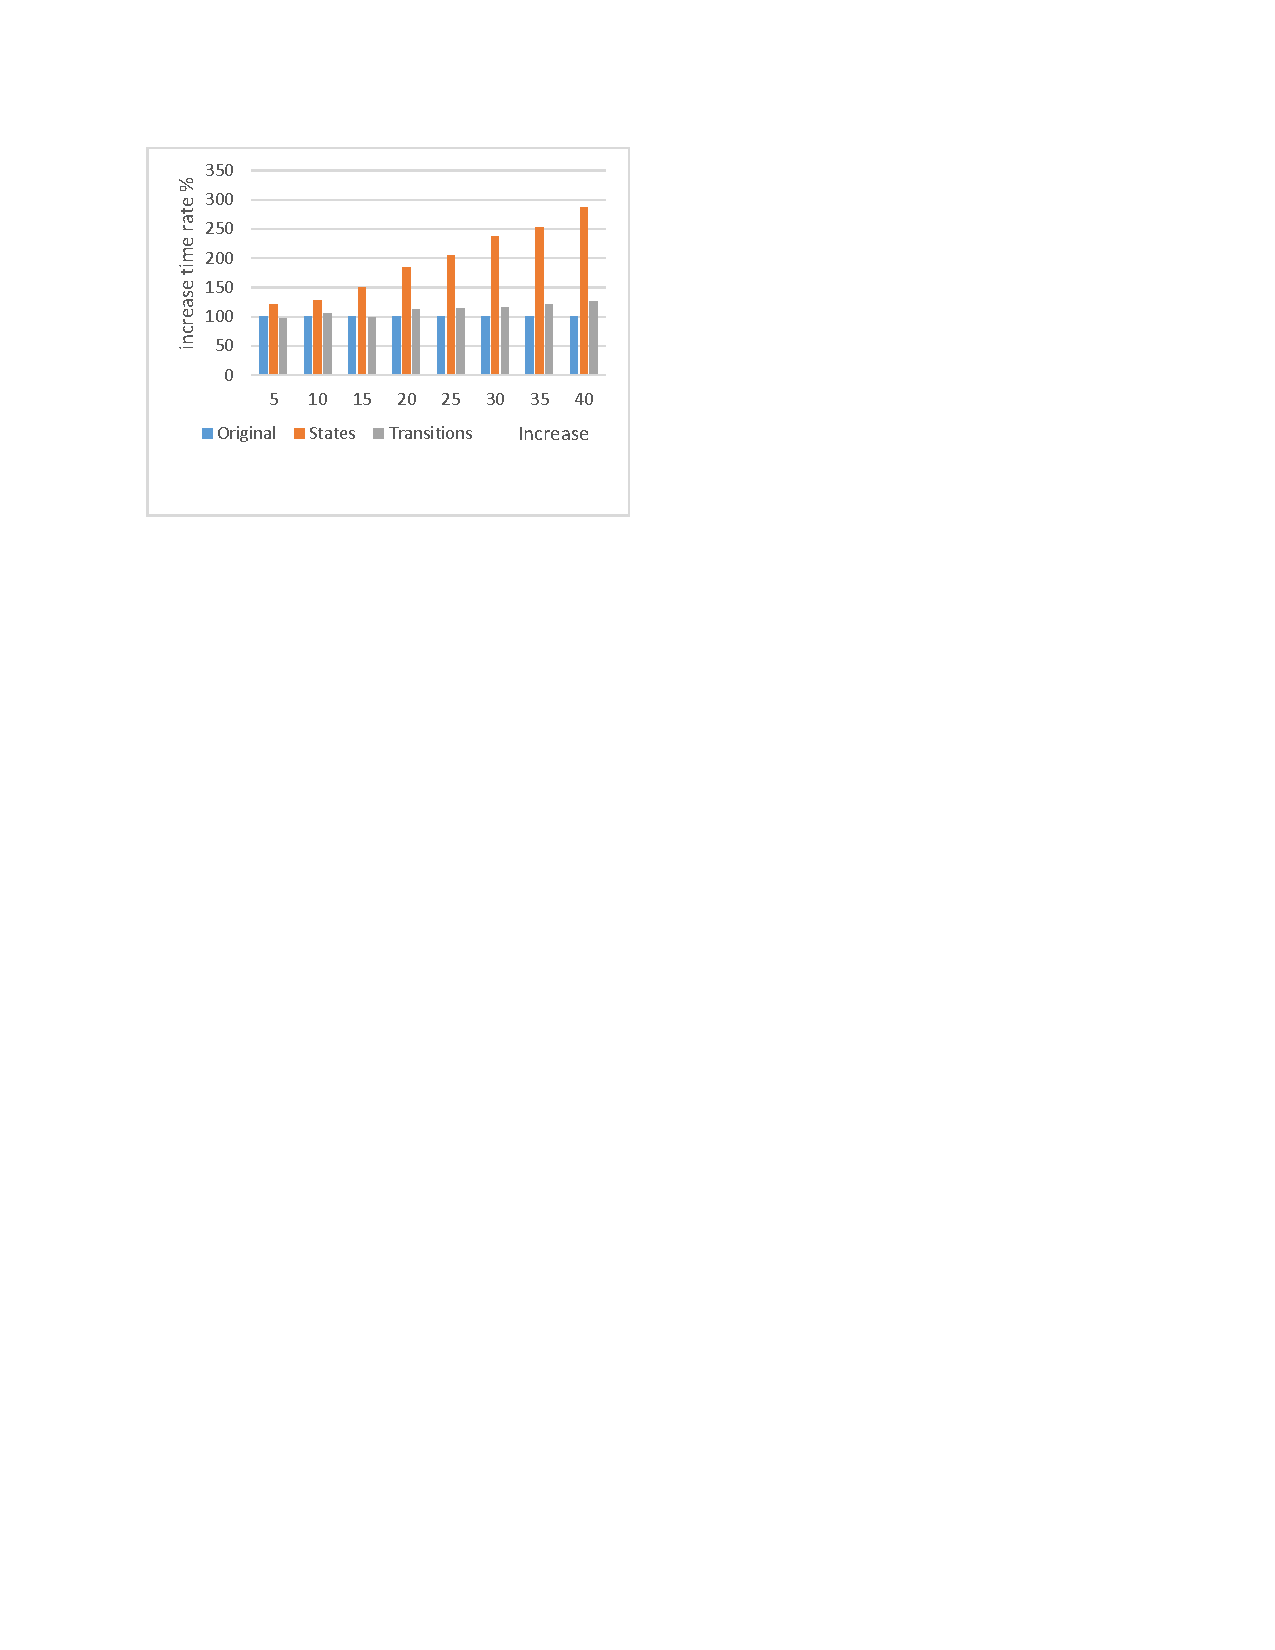
\includegraphics[clip, trim=3cm 20.5cm 11cm 2.6cm, width=0.5\textwidth]{figures/graph}
\caption{Impact comparison between states and transitions} 
\label{fig:graph}
\end{figure}

\subsection{Semantic conformance of runtime execution}
To evaluate the semantic conformance of runtime execution of generated code, we use a set of examples provided by Moka [XXX] which is a model execution engine offering Precise Semantics of UML Composite Structures \cite{OMG2015}. We compare the entered-ordered state list, which is obtained by simulating a state machine with the engine, with the state list obtained by the runtime execution of the generated code of the same state machine. The generated code is semantic-conformant if both of the lists are the same. [To be continued]

\subsection{Development/maintenance cost}
\label{subsec:cost}
To compare the development/maintenance cost, we investigate steps needed in generated code and models having the equivalent semantics. For example, to add a state, on one hand, two steps are needed in diagrams including (1) specifying the parent state and (2) dragging \& dropping the state notation to that parent. On the other hand, three code modifications are (1) create a state class inheriting from the base state and its constructors, (2) add to the parent state class an attribute, and (3) add a line of code to initialize the state attribute in the parent state constructor. Table \ref{table:cost} shows the number of steps needed for each operation. In this table, model manipulations are the winner in most of cases because of graphical representation advantages but code manipulations are still useful and comparable.

\begin{table}
\centering
\caption{Cost comparison}
\label{table:cost}
\begin{tabular}{|l|l|l|}
\hline
Description                                     & Model & Code \\ \hline
Add a state                                     & 2     & 3    \\ \hline
Add a transition                                & 3     & 3    \\ \hline
Add entry/exit action                           & 2     & 2    \\ \hline
Add transition action                           & 2     & 2    \\ \hline
Update action                                   & 1     & 1    \\ \hline
Redirect target state of a transition           & 1     & 1    \\ \hline
Create a call event to a transition & 3     & 6    \\ \hline
Create a time event to a transition & 3     & 5    \\ \hline
Delete a state                                  & 2     & 2    \\ \hline
Delete a transition                             & 1     & 3    \\ \hline
Delete entry/exit action                        & 1     & 2    \\ \hline
Delete transition action                        & 1     & 2    \\ \hline
Delete a call event                             & 2     & many \\ \hline
Delete a time event                             & 2     & many \\ \hline
\end{tabular}
\end{table}

In software development, programmers might modify the generated code, the modifications might violate structures of code or SM semantics. To resolve this issue, as previously described, we provide a semantic verification that partly and loosely inspects the AST of generated code. This inspection approach always reverses the code to the SM as well as the code is state machine-compliant even though the code is not compiled. This approach is very useful in practice in which programmers might partly modify code, automatically update the original SM by our RTRIP, and automatically re-generate state machine-compliant code into the remaining application code. This re-generation does no more than completing missing elements in code meaning that all previous changes are preserved. This practice is also limitedly supported by Fujaba \cite{KNNZ99_2_ag} in which activity and collaboration diagrams are partly synchronized with JAVA.




\section{Conclusion}
\label{sec:conclusion}
This paper presented a novel approach to round-trip engineering from UML state machines to code and back. The forward process of the approach is based on different patterns transforming UML state machine concepts such as states, transitions and events into an intermediate model containing UML classes. Object-oriented code is then generated from the intermediate model by existing code generators for programming languages such as C++ and JAVA. In the backward direction, code is analyzed and transformed into an intermediate whose format is close to the semantics of UML state machines. UML state machines are then straightforwardly constructed or updated from the intermediate format. 
 
The paper also showed the results of several experiments on different aspects of the proposed approach with the tooling prototype. Specifically, the experiments on the correctness of, the performance of, the semantic conformance of code generated by, and the cost of system development/maintenance using the proposed round-trip engineering are conducted. Although, the reverse direction only works if manual code is written following pre-defined patterns, the semantics of state machines is explicitly and intuitively present and easily to follow.

While the semantic conformance of code generated is critical, the paper only showed a lightweight experiment on this aspect. The reason is that the implementation of the prototype takes a lot of time. A systematic evaluation is therefore in future work. Furthermore, as evaluated in [7], the approach inheriting from the double-dispatch trades a reversible mapping for a slightly larger head. The reverse does not work concurrent state machine and several pseudo-states. Hence, future work should resolve these issues.

%\input{sections/ack}
\bibliographystyle{abbrv}
\bibliography{refs}

\end{document}
